\documentclass{ximera}
\graphicspath{  %% When looking for images,
{./}            %% look here first,
{./pictures/}   %% then look for a pictures folder,
{../pictures/}  %% which may be a directory up.
{../../pictures/}  %% which may be a directory up.
{../../../pictures/}  %% which may be a directory up.
{../../../../pictures/}  %% which may be a directory up.
}

\usepackage{listings}
%\usepackage{circuitikz}
\usepackage{xcolor}
\usepackage{amsmath,amsthm}
\usepackage{subcaption}
\usepackage{graphicx}
\usepackage{tikz}
%\usepackage{tikz-3dplot}
\usepackage{amsfonts}
%\usepackage{mdframed} % For framing content
%\usepackage{tikz-cd}

  \renewcommand{\vector}[1]{\left\langle #1\right\rangle}
  \newcommand{\arrowvec}[1]{{\overset{\rightharpoonup}{#1}}}
  \newcommand{\ro}{\texttt{R}}%% row operation
  \newcommand{\dotp}{\bullet}%% dot product
  \renewcommand{\l}{\ell}
  \let\defaultAnswerFormat\answerFormatBoxed
  \usetikzlibrary{calc,bending}
  \tikzset{>=stealth}
  




%make a maroon color
\definecolor{maroon}{RGB}{128,0,0}
%make a dark blue color
\definecolor{darkblue}{RGB}{0,0,139}
%define the color fourier0 to be the maroon color
\definecolor{fourier0}{RGB}{128,0,0}
%define the color fourier1 to be the dark blue color
\definecolor{fourier1}{RGB}{0,0,139}
%define the color fourier 1t to be the light blue color
\definecolor{fourier1t}{RGB}{173,216,230}
%define the color fourier2 to be the dark green color
\definecolor{fourier2}{RGB}{0,100,0}
%define teh color fourier2t to be the light green color
\definecolor{fourier2t}{RGB}{144,238,144}
%define the color fourier3 to be the dark purple color
\definecolor{fourier3}{RGB}{128,0,128}
%define the color fourier3t to be the light purple color
\definecolor{fourier3t}{RGB}{221,160,221}
%define the color fourier0t to be the red color
\definecolor{fourier0t}{RGB}{255,0,0}
%define the color fourier4 to be the orange color
\definecolor{fourier4}{RGB}{255,165,0}
%define the color fourier4t to be the darker orange color
\definecolor{fourier4t}{RGB}{255,215,0}
%define the color fourier5 to be the yellow color
\definecolor{fourier5}{RGB}{255,255,0}
%define the color fourier5t to be the darker yellow color
\definecolor{fourier5t}{RGB}{255,255,100}
%define the color fourier6 to be the green color
\definecolor{fourier6}{RGB}{0,128,0}
%define the color fourier6t to be the darker green color
\definecolor{fourier6t}{RGB}{0,255,0}

%New commands for this doc for errors in copying
\newcommand{\eigenvar}{\lambda}
%\newcommand{\vect}[1]{\mathbf{#1}}
\renewcommand{\th}{^{\text{th}}}
\newcommand{\st}{^{\text{st}}}
\newcommand{\nd}{^{\text{nd}}}
\newcommand{\rd}{^{\text{rd}}}
\newcommand{\paren}[1]{\left(#1\right)}
\newcommand{\abs}[1]{\left|#1\right|}
\newcommand{\R}{\mathbb{R}}
\newcommand{\C}{\mathbb{C}}
\newcommand{\Hilb}{\mathbb{H}}
\newcommand{\qq}[1]{\text{#1}}
\newcommand{\Z}{\mathbb{Z}}
\newcommand{\N}{\mathbb{N}}
\newcommand{\q}[1]{\text{``#1''}}
%\newcommand{\mat}[1]{\begin{bmatrix}#1\end{bmatrix}}
\newcommand{\rref}{\text{reduced row echelon form}}
\newcommand{\ef}{\text{echelon form}}
\newcommand{\ohm}{\Omega}
\newcommand{\volt}{\text{V}}
\newcommand{\amp}{\text{A}}
\newcommand{\Seq}{\textbf{Seq}}
\newcommand{\Poly}{\textbf{P}}
\renewcommand{\quad}{\text{    }}
\newcommand{\roweq}{\simeq}
\newcommand{\rowop}{\simeq}
\newcommand{\rowswap}{\leftrightarrow}
\newcommand{\Mat}{\textbf{M}}
\newcommand{\Func}{\textbf{Func}}
\newcommand{\Hw}{\textbf{Hamming weight}}
\newcommand{\Hd}{\textbf{Hamming distance}}
\newcommand{\rank}{\text{rank}}
\newcommand{\longvect}[1]{\overrightarrow{#1}}
% Define the circled command
\newcommand{\circled}[1]{%
  \tikz[baseline=(char.base)]{
    \node[shape=circle,draw,inner sep=2pt,red,fill=red!20,text=black] (char) {#1};}%
}

% Define custom command \strikeh that just puts red text on the 2nd argument
\newcommand{\strikeh}[2]{\textcolor{red}{#2}}

% Define custom command \strikev that just puts red text on the 2nd argument
\newcommand{\strikev}[2]{\textcolor{red}{#2}}

%more new commands for this doc for errors in copying
\newcommand{\SI}{\text{SI}}
\newcommand{\kg}{\text{kg}}
\newcommand{\m}{\text{m}}
\newcommand{\s}{\text{s}}
\newcommand{\norm}[1]{\left\|#1\right\|}
\newcommand{\col}{\text{col}}
\newcommand{\sspan}{\text{span}}
\newcommand{\proj}{\text{proj}}
\newcommand{\set}[1]{\left\{#1\right\}}
\newcommand{\degC}{^\circ\text{C}}
\newcommand{\centroid}[1]{\overline{#1}}
\newcommand{\dotprod}{\boldsymbol{\cdot}}
%\newcommand{\coord}[1]{\begin{bmatrix}#1\end{bmatrix}}
\newcommand{\iprod}[1]{\langle #1 \rangle}
\newcommand{\adjoint}{^{*}}
\newcommand{\conjugate}[1]{\overline{#1}}
\newcommand{\eigenvarA}{\lambda}
\newcommand{\eigenvarB}{\mu}
\newcommand{\orth}{\perp}
\newcommand{\bigbracket}[1]{\left[#1\right]}
\newcommand{\textiff}{\text{ if and only if }}
\newcommand{\adj}{\text{adj}}
\newcommand{\ijth}{\emph{ij}^\text{th}}
\newcommand{\minor}[2]{M_{#2}}
\newcommand{\cofactor}{\text{C}}
\newcommand{\shift}{\textbf{shift}}
\newcommand{\startmat}[1]{
  \left[\begin{array}{#1}
}
\newcommand{\stopmat}{\end{array}\right]}
%a command to give a name to explorations and hints and theorems
\newcommand{\name}[1]{\begin{centering}\textbf{#1}\end{centering}}
\newcommand{\vect}[1]{\vec{#1}}
\newcommand{\dfn}[1]{\textbf{#1}}
\newcommand{\transpose}{\mathsf{T}}
\newcommand{\mtlb}[2][black]{\texttt{\textcolor{#1}{#2}}}
\newcommand{\RR}{\mathbb{R}} % Real numbers
\newcommand{\id}{\text{id}}
\newcommand{\coord}[1]{\langle#1\rangle}
\newcommand{\RREF}{\text{RREF}}
\newcommand{\Null}{\text{Null}}
\newcommand{\Nullity}{\text{Nullity}}
\newcommand{\Rank}{\text{Rank}}
\newcommand{\Col}{\text{Col}}
\newcommand{\Ef}{\text{EF}}
\newcommand{\boxprod}[3]{\abs{(#1\times#2)\cdot#3}}

\author{Zack Reed}
%borrowed from Anna Davis and Gilbert Strang
\title{Fundamental Subspaces}\license{CC BY-NC-SA 4.0}

\begin{document}
\begin{abstract}

\end{abstract}
\maketitle

\section*{Column and Null Space of a Matrix}

In the previous activity we observed that the image of the linear transformation $T$ is the same as the span of the columns of the associated matrix $A$. We also saw that we could exactly describe the images of linear transformations, as well as their kernels (aka the null space of the associated matrix).

We're going to press further into exploring the spaces related to linear transformations' domains and co-domains, and get some simply stated and at times useful results.

This will involve re-stating some results from the previous sections but in formal definitions, and making more explicit that these sets are actual vector spaces in their own right, called \emph{subspaces}.

First, let's formally talk about the image of a transformation as the span of the column vectors from the associated matrix. This is called the \emph{column space} of the matrix.

\begin{definition}{Column Space}

The column space of the matrix $A$ is the span of its column vectors.

Since the column space directly determines the image of the associated transformation $T$, we can state that:

$$\mbox{im}(T)=\mbox{col}(A)$$
\end{definition}

Moreover, since $\mbox{im}(T)$ and $\mbox{col}(A)$ are the same space, they have the same dimension. We have a special word for the dimension of the column space, called the \emph{rank} of the matrix. 

\begin{definition}{Rank}

  The rank of a matrix $A$ is the dimension of its column space. You might also describe this as the rank of the transformation $T$, but this is less common. 

  As such, we have

$$\mbox{dim}(\mbox{im}(T))=\mbox{dim}(\mbox{col}(A))=\mbox{rank}(A)$$
\end{definition}
 
\begin{example}\label{ex:image2}
Let $T:\RR^5\rightarrow \RR^4$ be a linear transformation with standard matrix $$A=\begin{bmatrix}1 & 2 & 2 &-1 & 0\\-1 & 3 & 1 & 0 & -1\\3 & 0 & 0 & 3 & 6\\ 1 & -1 & 1 & -2 & -1\end{bmatrix}$$
Find $\mbox{im}(T)$ and $\mbox{rank}(A)$.

\begin{explanation}
As before, the image of $T$ is the column space of $A$, so we have 

$$\mbox{im}(T)=\mbox{span}\left(\begin{bmatrix}1\\-1\\3\\1\end{bmatrix}, \begin{bmatrix}2\\3\\0\\-1\end{bmatrix}, \begin{bmatrix}2\\1\\0\\1\end{bmatrix}, \begin{bmatrix}-1\\0\\3\\-2\end{bmatrix}, \begin{bmatrix}0\\-1\\6\\-1\end{bmatrix}\right)=\mbox{col}(A)$$

To better describe this, and see which vectors might be linear combinations of others, let's find \texttt{rref(A)}.
 
$$\text{rref}(A)=\begin{bmatrix} 1 & 0 & 0 & 1 & 2\\0 & 1 & 0 & 1 & 1\\0 & 0 & 1 & -2 & -2\\ 0 & 0 & 0 & 0 & 0 \end{bmatrix}$$
 
We can see that, more descriptively, the image is just the span of the first three vectors.

$$\mbox{im}(T)=\mbox{span}\left(\begin{bmatrix}1\\-1\\3\\1\end{bmatrix}, \begin{bmatrix}2\\3\\0\\-1\end{bmatrix}, \begin{bmatrix}2\\1\\0\\1\end{bmatrix}\right)$$
 
This also lets us determine $\mbox{rank}(A)$, which is $\answer{3}$. You might also notice that there were $\answer{3}$ pivot columns in \texttt{rref(A)}. This is no coincidence, and in fact you can quickly determine the rank of any matrix by counting the number of pivot columns in its \rref.
\end{explanation}
\end{example}
 
In the spirit of ``having many names for the same thing'', we have the following simple equation that shows agreement between the image of transformations and the column space of matrices.
 
\begin{formula}\label{form:rankTrankA}
$$\mbox{rank}(A) = \mbox{dim}(\mbox{col}(A))=\mbox{dim}(\mbox{im}(T))=\mbox{rank}(T)$$
\end{formula}
 
%Note that since  $\mbox{rank}(A) = \mbox{dim}(\mbox{col}(A))=\mbox{dim}(\mbox{im}(T))$, our definitions of the rank of a linear transformation and the rank of its associated standard matrix are in agreement.
 
\subsection*{Nullity and the Kernel of a Linear Transformation}
 
Before, we discussed how the \emph{kernel} of a linear transformation is all vectors that map to $\vec{0}$, that is, $\vec{v}$ such that $T(\vec{v})=\vec{0}$. For the sake of again using different verbiage for the same thing, it is worth stating that the kernel of a transformation is the null space of its matrix.

$$\mbox{ker}(T)=\mbox{null}(A).$$
 
\begin{example}\label{ex:kernel} Let $T:\RR^5\rightarrow \RR^4$ be a linear transformation with standard matrix $$A=\begin{bmatrix}1 & 2 & 2 &-1 & 0\\-1 & 3 & 1 & 0 & -1\\3 & 0 & 0 & 3 & 6\\ 1 & -1 & 1 & -2 & -1\end{bmatrix}$$
\begin{enumerate}
\item \label{item:kernelT}
Find $\mbox{ker}(T)$
\item \label{item:dimkernelT}
Find $\mbox{dim}(\mbox{ker}(T))$.
\end{enumerate}
\begin{explanation}

\ref{item:kernelT} We did this before, in the previous section, however it's always good to practice.
 
\texttt{rref(A)} yields:
 
$$\mbox{rref}(A)= \begin{bmatrix} 1 & 0 & 0 & 1 & 2\\0 & 1 & 0 & 1 & 1\\0 & 0 & 1 & -2 & -2\\ 0 & 0 & 0 & 0 & 0 \end{bmatrix}$$
 
From our work with null spaces, we can form vectors whose linear combinations form the kernel of $T$:
$$\mbox{ker}(T)=\begin{bmatrix}\answer{-1}\\-1\\\answer{2}\\\answer{1}\\0\end{bmatrix}s+\begin{bmatrix}\answer{-2}\\-1\\2\\0\\\answer{1}\end{bmatrix}t$$
 
We conclude that
$$\mbox{ker}(T)=\mbox{span}\left(\begin{bmatrix}\answer{-1}\\-1\\\answer{2}\\\answer{1}\\0\end{bmatrix},\begin{bmatrix}\answer{-2}\\-1\\2\\0\\\answer{1}\end{bmatrix}\right)$$
 
\ref{item:dimkernelT}  Since $\mbox{ker}(T)$ is the span of \wordChoice{\choice[correct]{two}\choice{three}\choice{five}} vectors of $\RR^5$, we can find the dimension of $\mbox{ker}(T)$. A quick check will determine that the \wordChoice{\choice[correct]{two}\choice{three}\choice{five}} spanning vectors are linearly independent, so we can see that $\mbox{dim}(\mbox{ker}(T))=\answer{2}$.

In fact, because of Gauss-Jordan elimination the spanning vectors are guaranteed to be linearly independent, so you can always assume that this method yields the entirety of the kernel (and hence the null space).
\end{explanation}
\end{example}
 
 
Recall that the \dfn{null space} of a matrix $A$ is defined to be set of all solutions to the homogeneous equation $A\vec{x}=\vec{0}$. This means that  if $T:\RR^n\rightarrow \RR^m$ is a linear transformation with standard matrix $A$ then
$$\mbox{ker}(T)=\mbox{null}(A)$$

\subsection*{Rank, Nullity, and Invertibility Conditions}

One of the more important uses of rank and nullity for the purposes of the current chapter is for determining whether nor not a transformation is invertible. Let's return to our initial example of the squished mug.

\begin{center}
  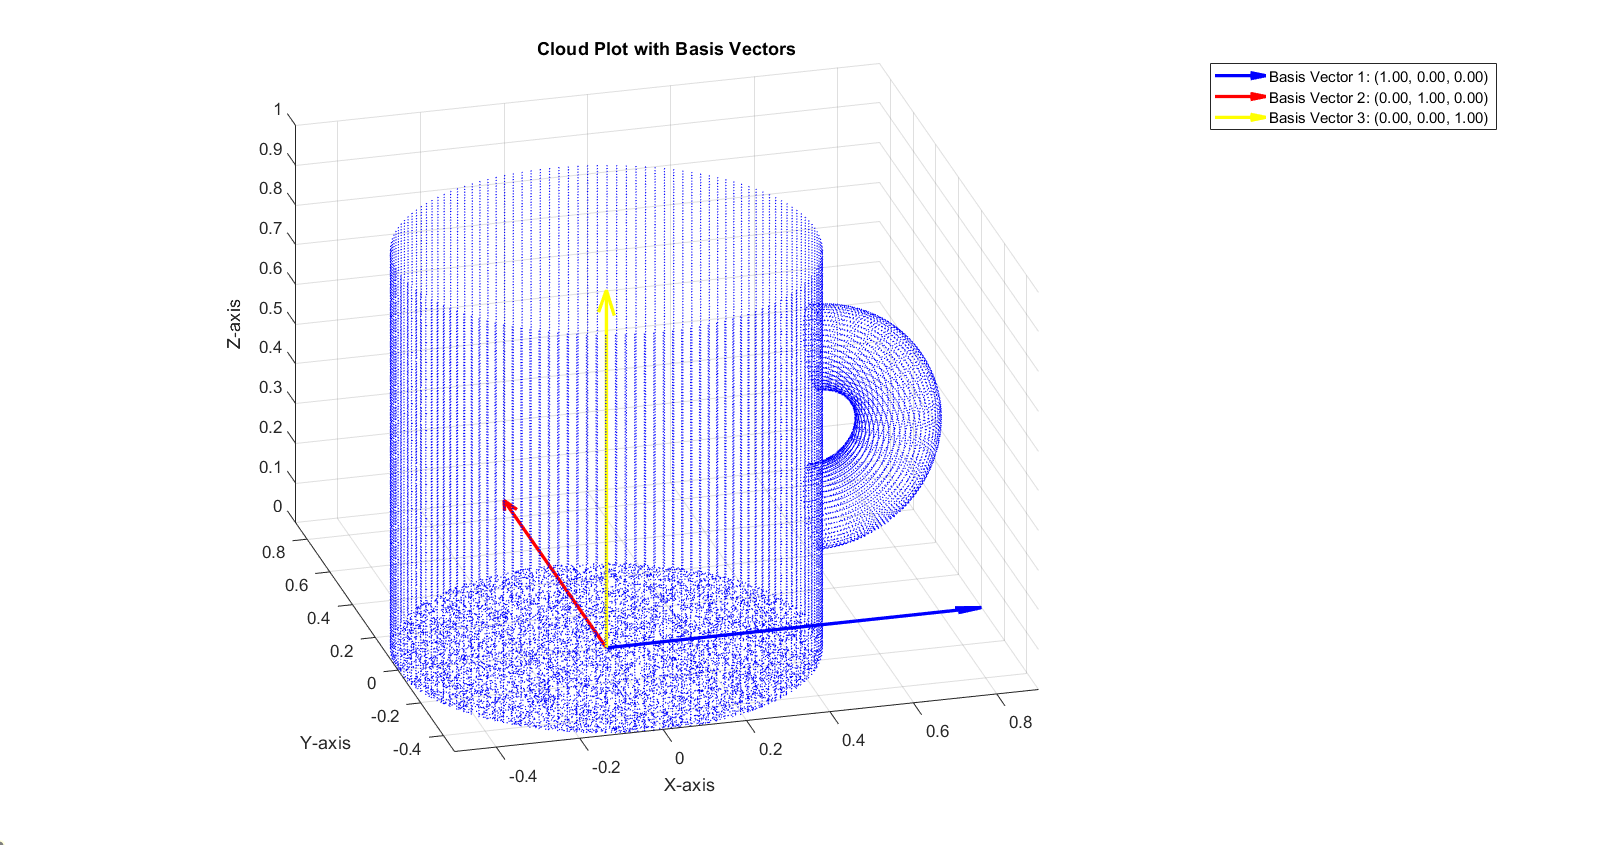
\includegraphics[width=20cm, height=16cm]{og_mug.png}
\end{center}

\begin{center}
  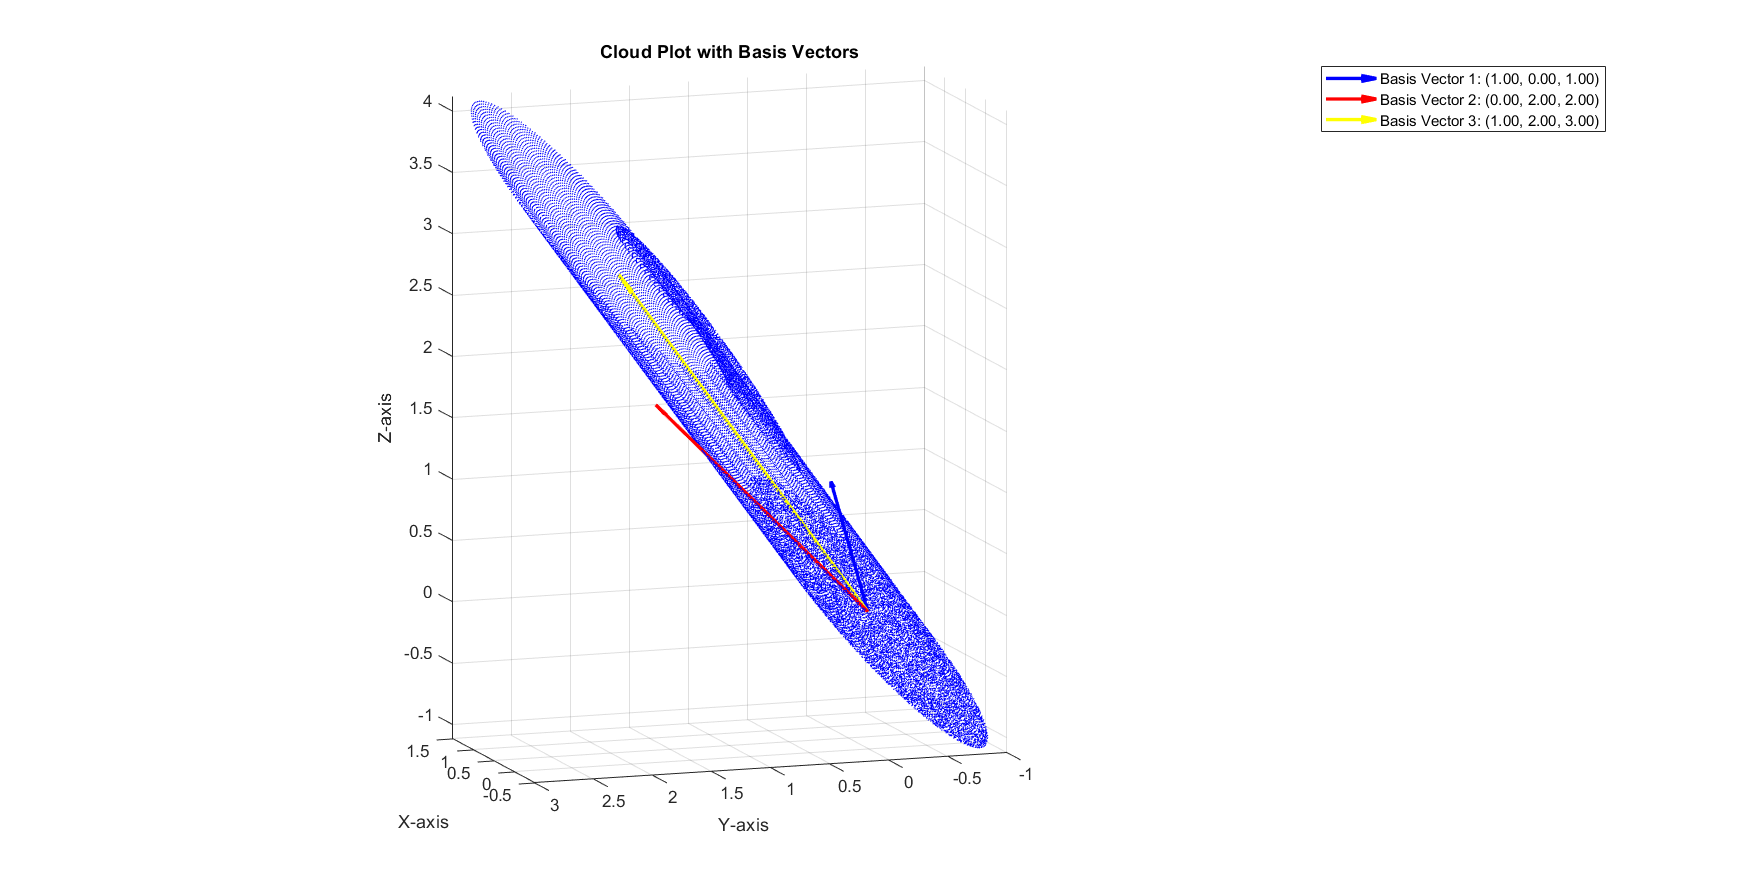
\includegraphics[width=20cm, height=16cm]{squished_mug.png}
\end{center}

The transformation $A=\begin{bmatrix}
  1&0&1\\0&2&2\\1&2&3
\end{bmatrix}$ fundamentally alters the mug by squishing it down to a plane. Even though the plane resides in $3D$ space, there is no linear transformation (nor no function more generally) that can take the squished mug vectors and return them to the original mug vectors. From a transformation perspective, this is because vectors in the plane would need to map to multiple mug vectors in space, for which there is no real systematic way to assign such a mapping. Considering images and null spaces, this suggests that if the dimension of the image is less than the dimension of the domain (e.g., the transformation squishes space) then the underlying matrix cannot be invertible. 

Accordingly, for a matrix to be invertible, we at least need that the dimensions of the image and the domain are the same. In fact, not only is this necessary, but this is actually all we need! If the dimension of the image is the same as the domain, then the columns of the matrix form a basis for the image space, and are hence linearly independent! Linear independence means that the $\texttt{rref}$ of the matrix is the identity, and so we have invertibility! 

The above loose argument roughly outlines one direction of the reasoning behind the more comprehensive theorem, stated here:

\begin{theorem}
  Let $A$ be an $n\times n$ matrix. The following are equivalent to each other (meaning if one is true, all are true):
  \begin{enumerate}
    \item $A$ is invertible.
    \item $A$ can be row-reduced to the identity (i.e. $\texttt{rref(A)}$ is $I$).
    \item $A$ has $n$ pivot positions.
    \item The rank of $A$ is $n$.
    \item The nullity of $A$ is $0$.
    \item The columns of $A$ form a basis for $\RR^n$.
    \item $A$ is a finite product of elementary matrices.
  \end{enumerate}
\end{theorem}

You now have a laundry list of conditions that can tell you whether a matrix is invertible. Breaking any one of these means the matrix breaks all of them, and is hence not invertible.
 

\end{document}